\documentclass[Space_Shuttle_Vessel_Manual.tex]{subfiles} 
\begin{document}

\section{SPACE SHUTTLE OVERVIEW}
\begin{multicols*}{2}
\label{sec:space-shuttle-overview}
\renewcommand{\cfttoctitlefont}{\bf}
\localtableofcontents
\noindent
\\
A small overview of the Space Shuttle is provided in this chapter. Further detail is available in the SCOM.
\end{multicols*} 

\subsection{Description}
\begin{figure}[b!]
  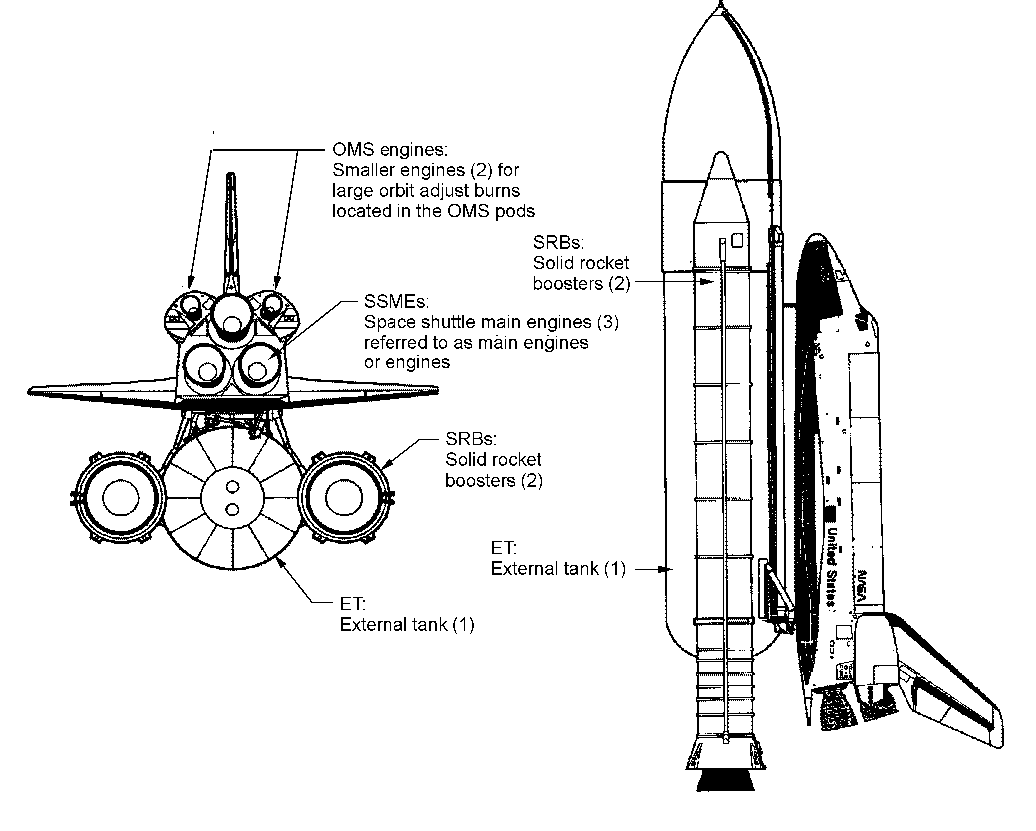
\includegraphics[width=1.0\textwidth]{stack.png}
  \caption{Space Shuttle}
  \label{fig:stack}
\end{figure}
\begin{multicols*}{2}
The Space Shuttle is a reusable space transportation system designed to launch and return payloads from Low Earth Orbit (LEO).\\
The main component is the Orbiter Vehicle (OV), which contains the major systems, crew and payload. For launch, the OV is attached to the External Tank (ET) which feeds the propellant to the 3 Space Shuttle Main Engines (SSME) in the OV. For further thrust during launch, 2 Solid Rocket Boosters (SRB) are attached to the ET.\\


\newpage

\subsection{Nominal Mission Profile}
\paragraph{Launch}
The launch is designed to guide the vehicle from the launch pad all to way to a pre-defined orbit. The SSMEs and SRBs are ignited on the pad, and fire together for about 2 minutes until the SRBs burnout and separate, ending what is know as "first stage". For the final 6 minutes of powered flight, called "second stage", the 3 SSMEs continue firing until the target velocity, and other parameters, are achieved. That point is called main engine cutoff (MECO). Shortly after MECO, the ET is separated, leaving the OV to fly the rest of the mission alone.\\
Although after MECO the OV is in space, it is a sub-orbital trajectory, and Orbital Maneuvering System (OMS) burns are required to finalize orbit insertion. The OMS-1 burn, about 2 minutes after MECO, is the first of the 2 orbit insertion burns, and it raises the apogee. The OMS-2 burn, about 45 minutes after launch at the apogee, raises the perigee. To increase payload mass, a "Direct Insertion" was developed, as opposed to the "Standard Insertion" described above, where MECO places the OV in an orbit such that the OMS-1 burn is not required.

\paragraph{Orbit}
After MECO, OV attitude control and small orbit changes are provided by the Reaction Control System (RCS), while large orbit changes are performed by the OMS.
The payload bay doors (PLBD) are opened early in the mission, so the radiators inside can cool the vehicle systems, while also allowing the payload operations to be performed. Mission objectives might call for a satellite deployment or retrieval, rendezvous and docking with a space station, scientific research in a pressurized module inside the PLB, or a combination of the above.
At the end of the mission, the PLBDs are closed for entry, and the OMS are used for a final burn to slow the vehicle down for entry into the atmosphere.

\paragraph{Entry}
Entry and landing are the final phases of the flight, guiding the OV from Entry Interface (EI) at 400k ft (121.92 km) all the way to an unpowered landing on a pre-selected runway. During the early phases of Entry, the vehicle is controlled by the RCS, but as the vehicle descends and the atmosphere gets more dense, the aerosurfaces begin to take over, and the usage of the RCS is eventually terminated.\\
The final approach to the runway is usually controlled by the Commander, which lands the vehicle and brakes to a stop. A drag chute was added to the OVs to help slowing down, thus decreasing loads on the brakes.\\
After the vehicle stops on the runway, a ground convoy approaches and work to turnaround the vehicle for another mission begins.
\end{multicols*}

\newpage
\subsection{Orbiter Vehicle (OV)}

\begin{figure}[b!]
  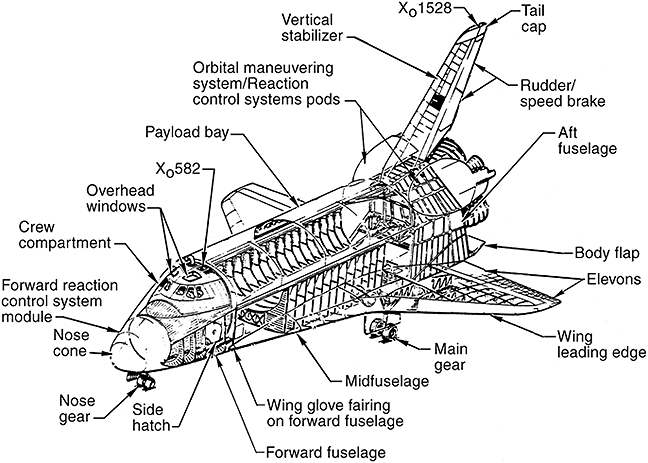
\includegraphics[width=1.0\textwidth]{OV.png}
  \caption{Orbiter Vehicle}
  \label{fig:OV}
\end{figure}
\begin{multicols*}{2}
The Orbiter Vehicle (OV) is the main part of the Space Shuttle.


The crew module, located in the forward fuselage, provides living space for up to 10 crew members, along with displays and controls for them to perform the mission.
The aft compartment contains the SSMEs and associated MPS equipment.
On-orbit attitude control is provided by the RCS, while aerosurfaces in the back of the wings and tail provide control in atmospheric flight.
Orbit change maneuvers are performed with the OMS engines, located on top of the aft compartment.\\
For protection during entry, the entire OV is covered with fragile tiles and blankets, which make up the Thermal Protection System (TPS).\\
The OV has a 15x60 ft (4.572 x 18.288 m) Payload Bay (PLB), which was designed to carry up to 65k lbs (29483.5 kg) of payload into orbit, and return 32k lbs (14514.96 kg) to Earth. Actual performance varied between OVs, as well as during the lifetime of the program.\\
For payload deploy and/or retrieval operations, the Remote Manipulator System (RMS) arm can be carried in the PLB. Post-Columbia accident flights carried the Orbiter Boom Sensor System (OBSS), which allows inspection of the TPS.\\
A total of 5 space-worthy OVs were build: OV-102 (Columbia), OV-099 (Challenger), OV-103 (Discovery), OV-104 (Atlantis) and OV-105 (Endeavour).\\


\subsubsection{Coordinate System}
\begin{figure}[H]
  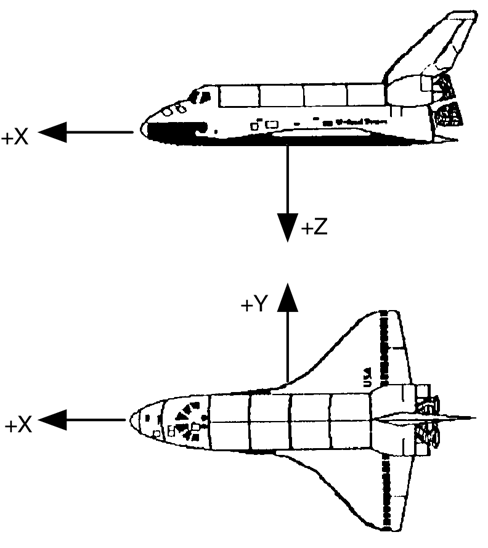
\includegraphics[width=0.5\textwidth]{ShuttleBodyAxisSystem.png}
  \caption{Body Axis Coordinate System}
  \label{fig:BodyAxisSystem}
\end{figure}
Figure \ref{fig:BodyAxisSystem} shows the shuttle Body Axis Coordinate system.\\
It should be noted that the Body Axis Coordinate frame is different from the normal Orbiter Space Flight Simulator frame.
% TODO replace ^^^ with something which also has PRY


\subsubsection{Main Propulsion System (MPS)}
The Main Propulsion System (MPS) is composed of the 3 SSMEs, that provide thrust during the whole launch, and propellant manifolds to feed propellants to the engines from their tanks in the ET.
\paragraph{Space Shuttle Main Engines (SSME)}
The SSMEs are high performance liquid propellant rocket engines located in the aft compartment of the orbiter. They can operate between 65\% and 109\% of their rated thrust, 370k lbf (1.646 MN), and are throttled down temporarily early in the ascent to reduce aerodynamic loads on the vehicle, and then again late in the ascent to keep the acceleration under 3g.
\paragraph{MPS Dump}
Following MECO and ET separation, the MPS Dump is automatically started to vent remaining MPS propellants from the engines and the manifolds. Liquid oxygen is vented thru the SSMEs and the liquid hydrogen is vented thru the backup LH2 dump valves and the LH2 fill and drain valves located on the port side of the OV.


\subsubsection{Auxiliary Power Unit/Hydraulics (APU/HYD)}
The OV has three independent hydraulic systems, each powered by an Auxiliary Power Unit (APU). Each system provides hydraulic pressure during launch and entry to control the SSMEs, the aerosurfaces, brakes and nose-wheel steering.\\
The APUs are started 5 minutes before launch and shut down shortly after MECO. The day before entry, a single APU is started for the FCS checkout. A single APU is started 5 minutes before the deorbit burn (this is done to ensure at least 1 APU is functioning before committing to entry). The remaining APUs are started 13 minutes before Entry Interface. All 3 APUs are shut down after landing.


\subsubsection{Orbital Maneuvering System (OMS)}
The Orbital Maneuvering System (OMS) is contained in 2 pods, located on the aft of the OV, each containing propellant tanks and an engine for large translation maneuvers in orbit. The OMS engines can be fired together or individually.


\subsubsection{Reaction Control System (RCS)}
The OV has 44 Reaction Control System (RCS) jets that provide for attitude control during the orbit and early entry phases of the flight, as well as small translation maneuvers in orbit.\\
The thrusters and associated propellant tanks are located in the nose of the OV and in the aft end of the OMS pods.


\subsubsection{Aerosurfaces}
The aerosurfaces allow control of the OV during atmospheric flight. They consist of 4 elevons, 2 on each wing, which provide pitch and roll control; a body flap in the aft compartment for elevon trim; a rudder in the vertical tail, made up of 2 panels, for turn coordination; and a speed brake, which opens the 2 rudder panels to create drag, allowing for energy control during the final approach to the runway.\\
Their movement is controlled with hydraulic actuators, powered by the 3 hydraulic systems.


\subsubsection{Payload Deploy and Retrieval System (PDRS)}
The Payload Deploy and Retrieval System consists of payload retention latches that hold large payloads inside the PLB, and the Remote Manipulator System (RMS) which allows for payload deploy and retrieval.

\paragraph{Remote Manipulator System (RMS)}
To deploy and retrieve payloads from the PLB the OV has a Canadian-built robotic arm know as the Remote Manipulator System (RMS). It has 6 joints allowing motion similar to the human arm. The End Effector (EE), located at the tip of the RMS, allows it to grapple payloads. The RMS can be moved in a single-joint mode, or moved along the axes of the OV or of the End Effector, thus allowing flexibility in its operation.\\
The RMS is positioned on the port side of the Payload Bay, mounted on the Manipulator Positioning Mechanism (MPM) that must be rolled out prior to RMS usage.


\subsubsection{Extra Vehicular Activities and Docking Operations Overview}
Extra Vehicular Activity (EVA), or spacewalk, is used on some missions for work outside the shuttle, either for retrieving a satellite or most recently, for the assembly of the ISS. Independently of mission tasks, all missions have contingency EVA capability for manual payload bay door closure. EVA requires the use of an airlock, which on the shuttle can be located inside the middeck (Internal Airlock), or outside on the payload bay (External Airlock). EVA is currently not supported by SSV.\\
For missions requiring docking with the ISS or Mir, the orbiter need to be fitted with the Orbiter Docking System (ODS). The ODS is mounted on top of the External Airlock, and is controlled from panel A7L, allowing ODS powerup and docking ring extension and retraction.\\
\\
\WARNING{A future version of SSV will introduce changes to the docking port format. In addition to the docking port, there must exist an child attachment, in the same location, with the id "APAS" to achieve soft-docking. Without the attachment, docking will not be possible.}\\
\\
\\
For missions requiring the ODS to be located aft of its normal position (e.g. STS-88), the Tunnel Adapter Assembly (TAA) is positioned between the External Airlock and the forward bulkhead, effectively acting as a spacer. The TAA must also be used on missions carrying the Spacelab or the SpaceHAB modules. It must be placed at the forward end of the tunnel to provide a way in/out of the airlock during an EVA.


\subsubsection{Crew Compartment Location Codes}
Crew Compartment location codes enable crew members to locate displays and controls, stowage compartments and lockers, access panels, and wall-mounted equipment in the OV crew compartments. The crew compartments are the flight deck, middeck, and airlock. Because of compartment functions and geometry, each has a unique location coding format.
\\
A flight deck location code consists of two or three alphanumeric characters. The first character is the first letter of a flight deck surface as addressed while sitting in the commander/pilot seats.
The second and third characters are numbers identifying the relative location of components on each flight deck surface. Table \ref{tab:PanelNumbering} lists the surfaces and the numbering philosophy for each surface.
Figures \ref{fig:FlightDeckLocCodes1} and \ref{fig:FlightDeckLocCodes2} show the flight deck panels and their location codes.
\begin{table}[H]
  \begin{tabularx}{\linewidth}{l | X}
    SURFACES & NUMBERING PHILOSOPHY \\
    \hline
    L - Left & \multirow{3}{\linewidth}{Numbered from top to bottom, forward to aft} \\
    R - Right & \\
    C - Center Console & \\
    \hline
    O - Overhead & Numbered from left to right, forward to aft \\
    \hline
    F - Forward & \multirow{2}{\linewidth}{Numbered left to right, top to bottom (facing the surface)} \\
    A - Aft & \\
    \hline
    \multirow{3}{*}{W - Windows} & \textbf{Forward} (W1 through W6): numbered left to right facing forward \\
    & \textbf{Overhead} (W7 \& W8): numbered left to right facing aft \\
    & \textbf{Aft} (W9 \& W10): numbered left to right facing aft \\
    \hline
    S - Seats & CDR seat is S1, PLT seat is S2, S3 and S4 are also in the flight deck, the rest in the middeck
  \end{tabularx}
  \caption{Flight Deck Numbering scheme}
  \label{tab:PanelNumbering}
\end{table}
\end{multicols*}

\newpage
\begin{figure}[H]
  \centering
  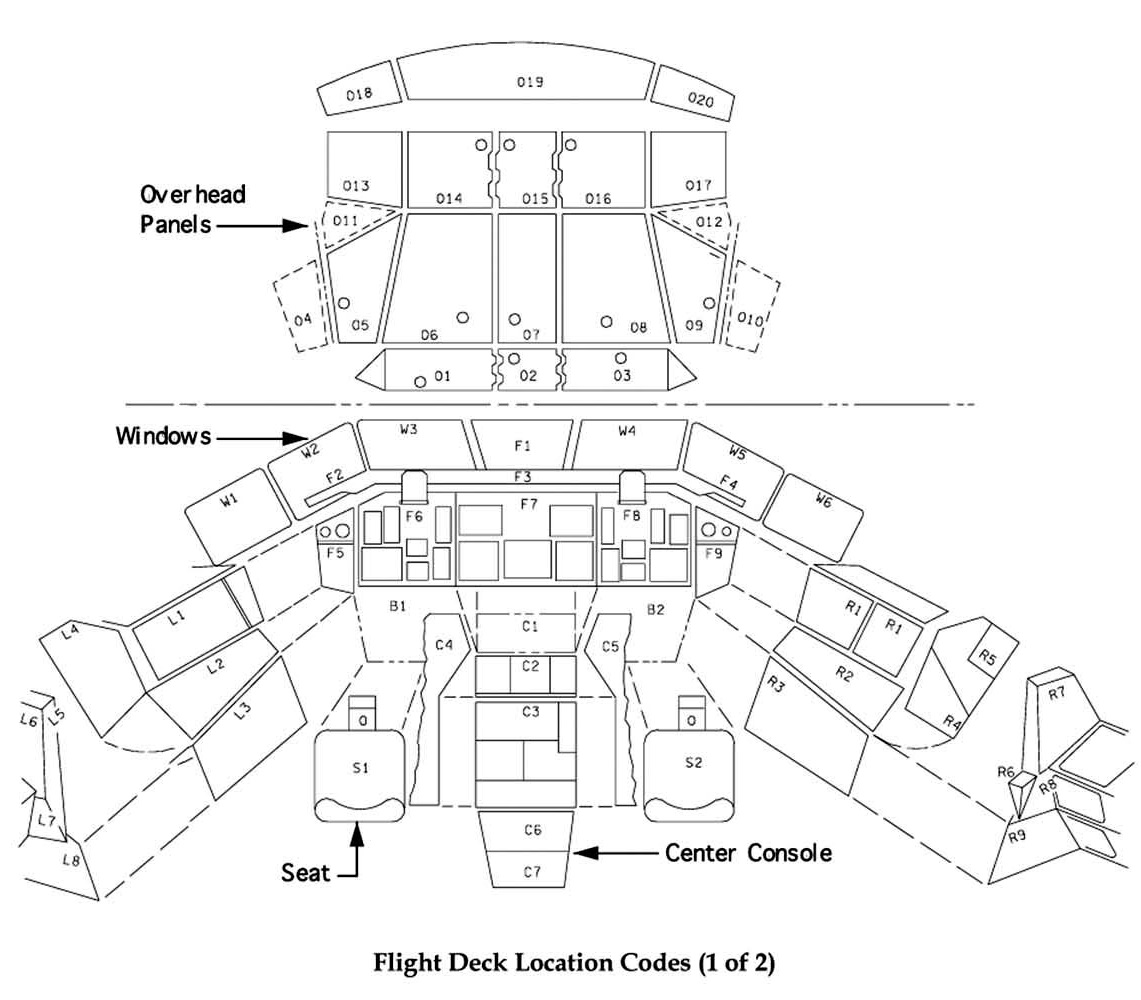
\includegraphics[width=\textwidth,height=0.5\textheight,keepaspectratio]{Flight_Deck_Loc_Codes_1.jpg}
  \caption{}
  \label{fig:FlightDeckLocCodes1}
\end{figure}
\begin{figure}[H]
  \centering
  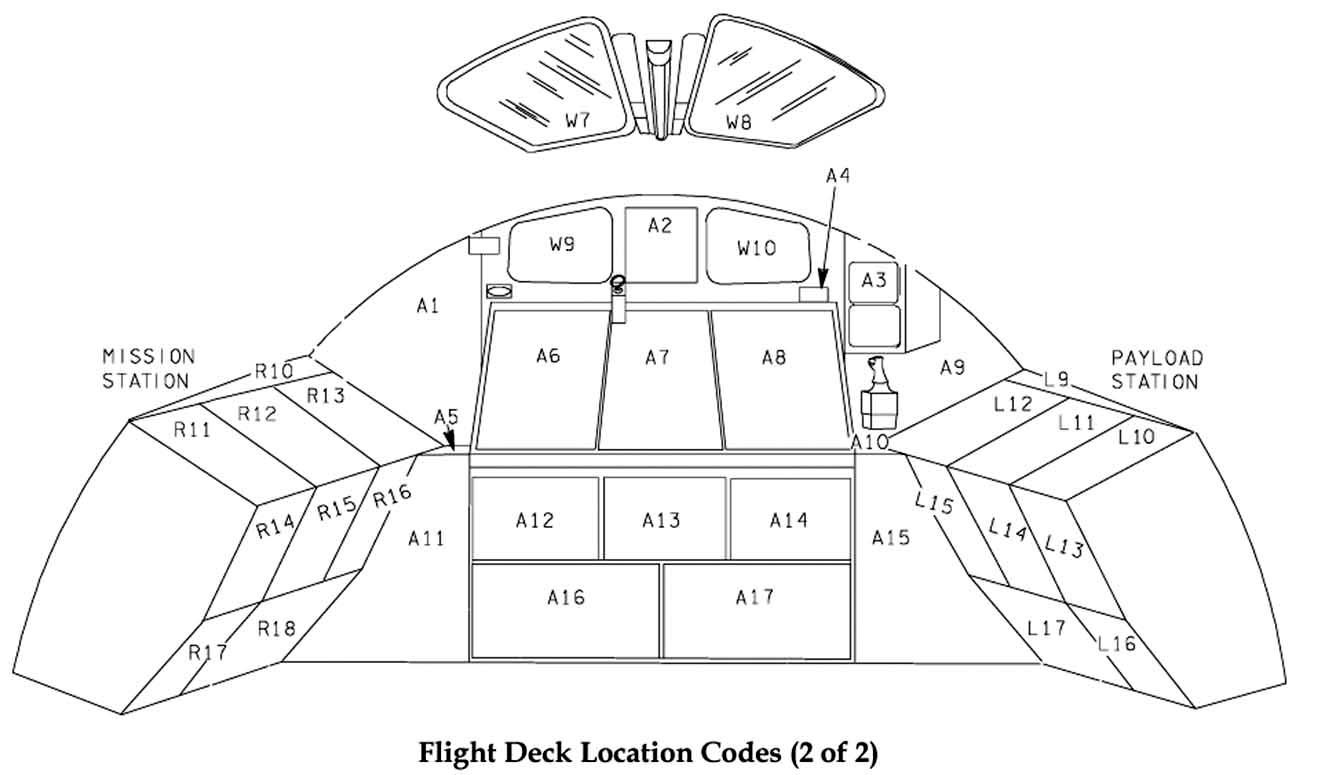
\includegraphics[width=\textwidth,height=0.35\textheight,keepaspectratio]{Flight_Deck_Loc_Codes_2.jpg}
  \caption{}
  \label{fig:FlightDeckLocCodes2}
\end{figure}






\subsection{External Tank (ET)}
\begin{figure}[b!]
  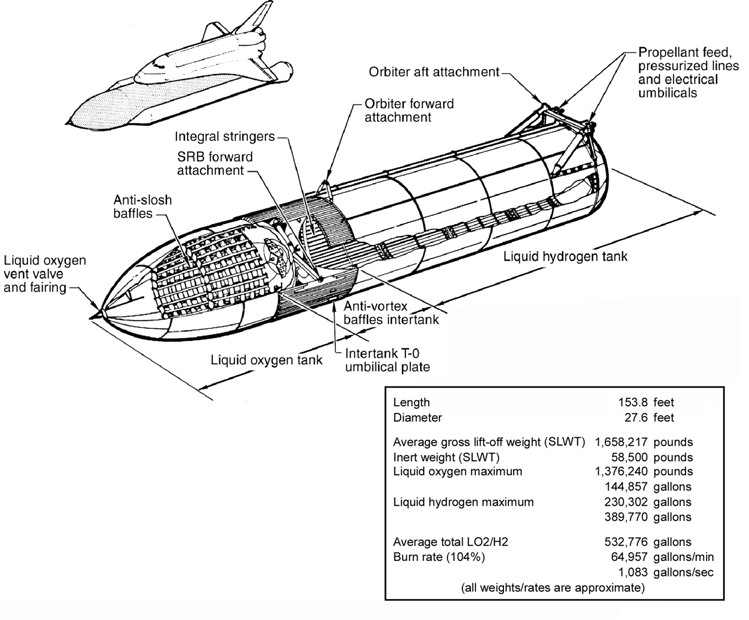
\includegraphics[width=1.0\textwidth]{SLWT.png}
  \caption{External Tank}
  \label{fig:ET}
\end{figure}
\begin{multicols*}{2}
The External Tank (ET) holds the liquid hydrogen and liquid oxygen propellants for the Main Propulsion System, and serves as a backbone for the whole Space Shuttle vehicle during launch. It separates from the OV about 8 minutes and 30 seconds after launch. The ET is the only major component of the Space Shuttle that is not reusable, and burns up in the atmosphere following launch. To keep the cryogenic propellants from boiling, the ET is covered in spray-on foam insulation.\\
A total of 3 versions of the ET were build$\colon$\\
$\Rightarrow$ Standard Weight Tank (SWT), the original design of the ET. For the first 2 flights it was painted with Fire Retardant Latex (FRL) paint, giving it a white color;\\
$\Rightarrow$ Light Weight Tank (LWT), a lighter weight ET resulting from structural changes;\\
$\Rightarrow$ Super Light Weight Tank (SLWT), further weight reductions to improve payload capability.\\
\end{multicols*}




\subsection{Solid Rocket Boosters (SRB)}
\begin{figure}[b!]
  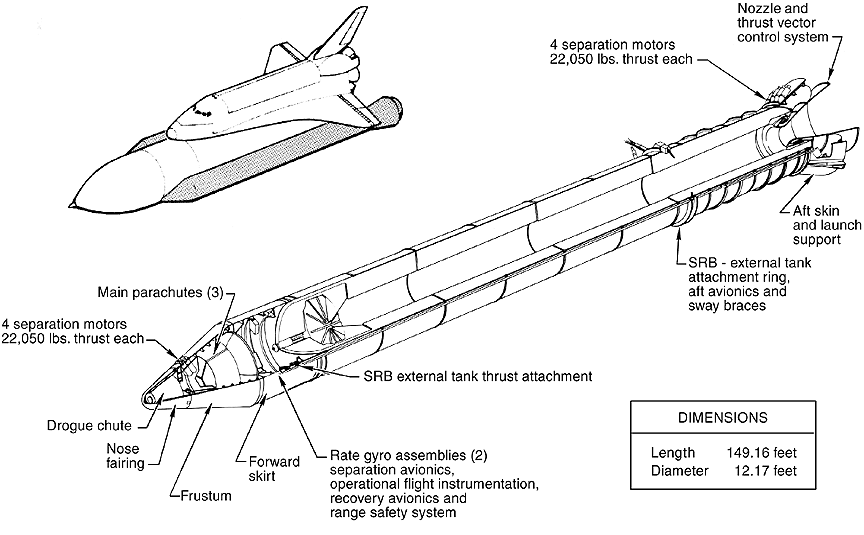
\includegraphics[width=1.0\textwidth]{SRB.png}
  \caption{Solid Rocket Booster}
  \label{fig:SRB}
\end{figure}
\begin{multicols*}{2}
The Solid Rocket Boosters (SRB) are solid propellant rockets that provide the majority of the thrust during the early phases of the launch, separating when their propellant is exhausted at about 2 minutes after launch. Following separation, they parachute down to the ocean not far from the launch site, are recovered and refurbished for another launch.\\
The main component of the SRB is the Solid Rocket Motor (SRM), a 4-segment solid-propellant rocket.\\
There are 4 types of SRMs$\colon$\\
$\Rightarrow$ Standard Performance Motor (SPM), the original SRM;\\
$\Rightarrow$ High Performance Motor (HPM), a lower-mass and higher-thrust upgrade to the SPM;\\
$\Rightarrow$ Filament Wound Case (FWC), a lighter, composite case SRM planned to be used from SLC-6;\\
$\Rightarrow$ Redesigned Solid Rocket Motor (RSRM), developed in response to the Challenger accident.\\
\end{multicols*}


\end{document}